\documentclass[11pt,a4paper]{report}

\usepackage[T1]{fontenc}
\usepackage[utf8]{inputenc}
\usepackage[english]{babel}
\usepackage{lmodern}
%\usepackage{circuitikz}
\usepackage{color}
\usepackage{wrapfig}
\usepackage{placeins}
\usepackage{subfigure}
\usepackage{tabu}
\usepackage{fullpage}
\usepackage[squaren]{SIunits}
\usepackage{graphicx}
%\usepackage[pdftex]{graphicx}
\usepackage{epstopdf}
\usepackage{epsfig}
\usepackage{hyperref}
\usepackage{tikz}
\usepackage{tikz-qtree}
\usepackage{eurosym}
%\usepackage{chemist}
\usepackage{amsmath}
\usepackage{amssymb}
\usepackage{mathrsfs}
\usepackage{dsfont}% use $\mathds{1}$
\newcommand{\C}{\mathbb{C}}
\newcommand{\N}{\mathbb{N}}
\newcommand{\Z}{\mathbb{Z}}
\newcommand{\R}{\mathbb{R}}
\newcommand{\red}{\textcolor{red}}
\newcommand{\dis}{\displaystyle}
\newcommand{\dr}{\partial}
\newcommand{\txt}{\text}
\newcommand{\td}{\todo[inline]}
\newcommand{\ttt}{\texttt}
\newcommand{\itt}{\textit}

\usepackage{algorithm}
\usepackage{todonotes}
\usepackage[noend]{algpseudocode}

%\newtheorem{theoreme}			     {Théorème}	[chapter]
%\newtheorem{proposition}[theoreme]	 {Proposition}	
%\newtheorem{corollaire}	  [theoreme]	 {Corollaire}	
%\newtheorem{lemme}	      [theoreme]  {Lemme}		
%\newtheorem{definition}	         {Définition}[chapter]
%\theoremstyle{definition}
%\newtheorem{exemple}			     {Exemple}	[chapter]
%\newtheorem{contreexemple}[exemple]{Contre-exemple}
%\newtheorem{probleme}	             {Probl\`eme}[chapter]

\usepackage{listings}
\usepackage{textcomp}
\definecolor{listinggray}{gray}{0.9}
\definecolor{lbcolor}{rgb}{0.9,0.9,0.9}
\lstset{
	backgroundcolor=\color{lbcolor},
	tabsize=4,
	rulecolor=,
	language=matlab,
        basicstyle=\scriptsize,
        upquote=true,
        aboveskip={1.5\baselineskip},
        columns=fixed,
        showstringspaces=false,
        extendedchars=true,
        breaklines=true,
        prebreak = \raisebox{0ex}[0ex][0ex]{\ensuremath{\hookleftarrow}},
        frame=single,
        showtabs=false,
        showspaces=false,
        showstringspaces=false,
        identifierstyle=\ttfamily,
        keywordstyle=\color[rgb]{0,0,1},
        commentstyle=\color[rgb]{0.133,0.545,0.133},
        stringstyle=\color[rgb]{0.627,0.126,0.941},
}

\DeclareMathOperator{\e}{e}

\title{Titre}
\author{Florentin Goyens}
\date{\today}

\begin{document}
\tabulinesep=1.2mm
\begin{center}
\hrule
\begin{tabular}{c}
\\[0.005cm]
\Large{Applied Numerical Methods - Lab 4}\\[0.3cm]
\textsc{Goyens} Florentin  \& \textsc{Weicker} David\\[0.2cm]
$\text{6}^{\text{th}}$ November 2015\\[0.2cm]
\end{tabular}
\hrule
\end{center}


\section*{Stationary heat conduction in 1-D}

In a one dimensional pipe we are interested in the temperature evolution along the z-axis.  We will study the behaviour of the numerical solution based on finite differences.



\subsection*{a) Reformulation of the problem}

We apply the change of variable $T=T_{0}u$, $x=L\xi$ and $t=t_{p}\tau$. This gives 
$$\dfrac{\partial T}{\partial t } = \dfrac{\partial T}{\partial \tau }\dfrac{\partial \tau}{\partial t }= \dfrac{T_0}{t_p}\dfrac{\partial u}{\partial \tau },$$
and similarly 
$$\dfrac{\partial^2 T}{\partial x^2} =  \dfrac{T_0}{L^2} \dfrac{\partial^2 T}{\partial \xi^2}.$$

So the equations becomes 
$$\rho C_p \dfrac{T_0}{t_p}\dfrac{\partial u}{\partial \tau } = k \dfrac{T_0}{L^2} \dfrac{\partial^2 u}{\partial \xi^2 }.$$
Writing 
$$ \dfrac{\partial u}{\partial \tau } =  \dfrac{k}{rho C_p L^2} \dfrac{\partial^2 u}{\partial \xi^2 }.$$
We have $a=\dfrac{t_p k}{\rho C_p L^2}$ and we check that it has no dimension, $\dfrac{s \cdot J/(m \cdot s \cdot C) }{kg/m^3 \cdot J/(kg \cdot C) \cdot m^2}$.








  


\subsection*{b) Discretize to a system of equation}

Points go from $\xi_{0}$ to $\xi_m$ and there is a ghost point at $\xi_{m+1}$.

$$\dfrac{du}{dt}= \dfrac{U_{i+1}-2U_{i}+U_{i-1}}{h^2} \text{ for } i= 1, .., N.$$

and the right boundary condition is $\dfrac{\partial u}{\partial \xi}=0$. We approximate with $(U_{m+1}-U_{m})/2h^2 = 0$ or $U_{m+1}=U_{m}$.



$$\dfrac{du}{dt}= \dfrac{1}{h^2}
\begin{pmatrix}
-2  & 1 &        &         &  & \\
1 & -2 & 1 &         &  & \\
       & 1 & \ddots & \ddots  &  & \\
       &        & \ddots &         &   &    \\
	   &        &        & 1 & -2 & 1\\
	   &			&		&		  & 2 & -2
\end{pmatrix}U + \dfrac{1}{h^2}\begin{pmatrix}
x\\
0\\
\vdots \\
0
\end{pmatrix}$$



\subsection*{c) Resolution}

Let us now use Euler's explicit method to solve the equation $\dfrac{dU}{d \tau}= AU+b(\tau)$ in time. The scheme gives
\begin{align*}
U^{k+1} &= U^{k} + \Delta t\Big(\dfrac{1}{h^2}AU^{k}+\dfrac{1}{h^2}b(\tau)\Big)\\
 &= \Big( I_{N} + \dfrac{\Delta t}{h^2} A\Big)U^{k} + \dfrac{\Delta t}{h^2}\cdot b(\tau)
\end{align*}
The code is available below in \ttt{tempEE.m}.

We cannot choose $\Delta x$ and $\Delta t$ as we want to obtain a stable solution.The following tests have been made :

\begin{center}
\begin{tabular}{|c|c|c|c|}
\hline 
$\Delta x$ & $\Delta t$ &$\frac{\Delta t}{\Delta x^2}$ &\textbf{Stability} \\ 
\hline 
0.05 & 0.01 &4 &Unstable \\ 
\hline 
 0.1& 0.001 & 0.1 &Stable \\ 
\hline 
0.1 & 0.005 & 0.5 &Stable \\ 
\hline 
0.1 &0.0051 &0.51 &Unstable\\
\hline
\end{tabular} 
\end{center}

It is possible to show that, in order to have a stable solution, the following condition must be satisfied : $\frac{\Delta t}{\Delta x^2} \leq \frac{1}{2}$.

We present a stable and an unstable solution on the figures~\ref{fig:stable},\ref{fig:unstable}.
They were obtained respectively with the calls \ttt{tempEE(10,0.005,2)} and \ttt{tempEE(10,0.0051,2)}. This corresponds to $\Delta x = 0.1$ and $\Delta t = \{0.005, 0.0051 \}$. This gives $\dfrac{\Delta t}{\Delta x^2}= \{0.5,0.51\}$. The unstable case breaks the condition $\dfrac{\Delta t}{\Delta x^2}\leq \dfrac{1}{2}$.

We can clearly see that the solution presented in figure \ref{fig:unstable} is unstable. Indeed, it shows large oscillations and even negative temperatures (which is not possible since the rod is heated).

\begin{figure}[!h]
\centering
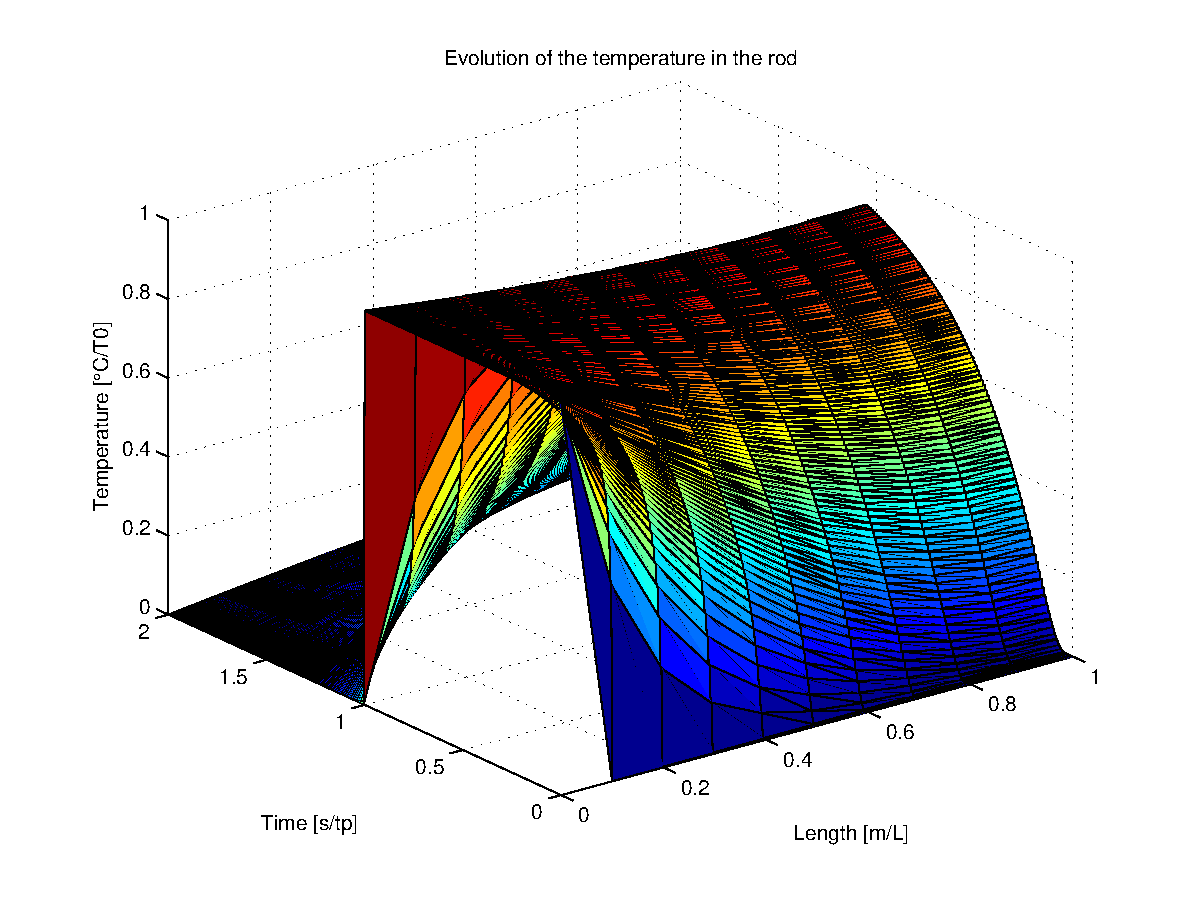
\includegraphics[width = 0.7\textwidth]{./stable.eps}
\caption{Stable solution }
\label{fig:stable}
\end{figure}

\begin{figure}[!h]
\centering
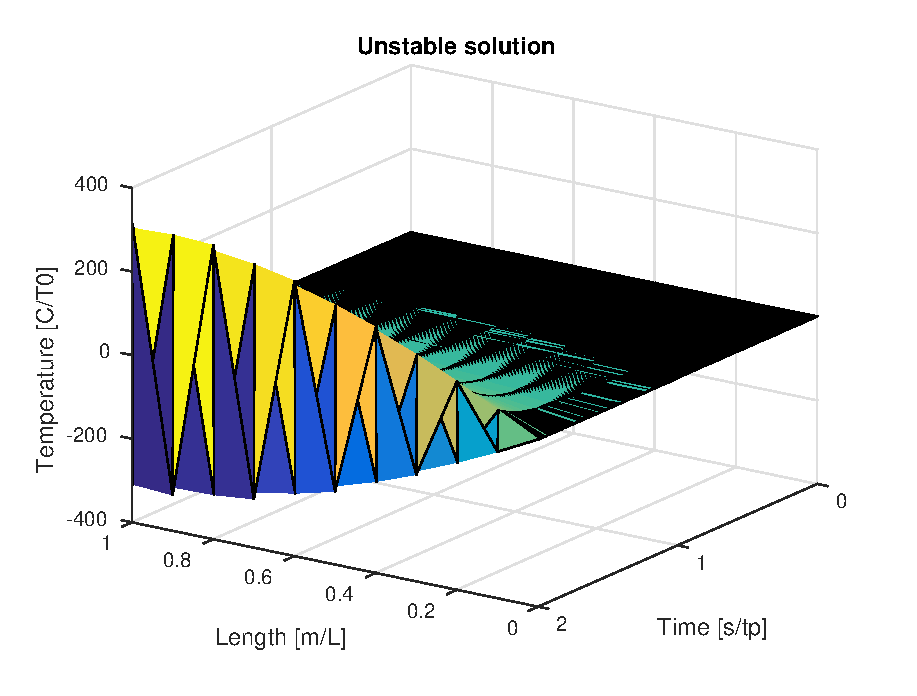
\includegraphics[width = 0.7\textwidth]{./unstable.eps}
\caption{Unstable solution }
\label{fig:unstable}
\end{figure}
\FloatBarrier


\subsection*{d) Comparison of methods}

In this section, we will compare two methods for solving the system of differential equations (the one obtained in part 2) : the explicit method $ode23$ and the implicit method $ode23s$. As already said, an implicit method is often more suitable for stiff problems.

The two methods will be compared for differents constant stepsizes for the spatial discretization ($N \in [10,20,40]$) and for a determined time interval ($\tau \in [0;2]$). We will based our analysis our three different factors : the number of steps needed to reach $\tau = 2$, the cpu-time needed to do the computations and the maximal value of the stepsize for the time discretization. The default tolerances are used for both methods.

The Matlab code used to do this analysis can be found at the end of this section. As we will reuse this code for part e, this is how the function was called : 
$$[timeStep,cpuTime,hMax] = tempOde('Gaussian')$$

The returned variables are arrays containing the data. The first column is when $ode23$ is used and the second is for $ode23s$. The lines correspond to the different stepsizes for the spatial discretization.

The call to this function gives the following data : 

\begin{center}
\begin{tabular}{|c|c|c|c|}
\hline 
  & \textbf{timesteps} & \textbf{cpu - time} & \textbf{h}$_{tmax}$ \\ 
\hline 
$N$ & $ode23 \phantom{fedz} ode23s$ & $ode23 \phantom{fedz} ode23s$ & $ode23 \phantom{fedz} ode23s$ \\ 
\hline 
10 &345 \phantom{fedzf} 104  & 0.1479 \phantom{fedz}    0.1944 &  0.0169  \phantom{fedz}  0.1473 \\ 
\hline 
20 & 1295 \phantom{fedz} 132 & 0.4730  \phantom{fedz}  0.4108 & 0.0043  \phantom{fedz}  0.1563 \\ 
\hline 
40 & 5114 \phantom{fedz} 169 &1.9056 \phantom{fedz}   0.8883  & 0.0010  \phantom{fedz}  0.1522 \\ 
\hline 
\end{tabular} 
\end{center}


We can easily see that, for all the factors taken into account, $ode23s$ is better than its explicit counterpart. 

First, the number of time steps. The explicit method needs much more steps to reach $\tau = 2$, this is because the problem is stiff. We can even compare this number with the theoretical number needed for stability in the case of a constant step size. For $N=10$, the maximal stable stepsize would be $h_t = \frac{(0.1)^2}{2} = 0.005$ so the number of steps to reach $\tau=2$ would be $n = \frac{2}{0.005} = 400$. We can see that $ode23$ is just a little better whereas $ode23s$ divides this number by 4.

Concerning the cpu - time, $ode23s$ is an obvious winner only when $N=40$. For $N=10$, $ode23$ is even a little bit better. This is mainly because the Gaussian elmination of the linear system takes time, but this will be solved in part e.

Finally, the maximal timestep looks approximately constant for $ode23s$. This is not the case for the explicit method. It has to reduce considerably the timestep in order to avoid instability.

\subsection*{e) Improvements}

In this section, we will try to improve the efficiency of $ode23s$. Indeed, this method has, at each timestep, to solve a system and uses a Gaussian elimination. However, our system is tridiagonal so this is not optimal. It is in fact possible to "tell" Matlab a bit more about our system so that the resolution will be more efficient. Two ways are used here. 

First, we can tell him which entries of the jacobian are non zeros. It will increase the efficiency because Matlab will know what computations are not necessary (because somothing times zero is always zero). This is done by the $odeset$ property called $JPattern$. We can obtain information by calling the same function as in part d but with a different argument : 
$$[timeStep,cpuTime,hMax] = tempOde('sparse')$$

Second, we can tell Matlab what is the jacobian of our system. In our case, it is a constant matrix. This will greatly help Matlab in his resolution of the system. To see this, we can call : 
$$[timeStep,cpuTime,hMax] = tempOde('jacobian')$$

To see the effect of the combined properties, we can call : 
$$[timeStep,cpuTime,hMax] = tempOde('both')$$

The following table contains the cpu - time for $N=10,20,40$ for different combinations of the $odeset$ properties with the method $ode23s$. The column $'both'$ means that the two properties were set.

\begin{center}
\begin{tabular}{|c|c|c|c|c|}
\multicolumn{5}{c}{\textbf{CPU - time} $(ode23s)$} \\
\hline 
 N& Gaussian & sparse & jacobian & both \\ 
\hline 
10 & 0.1944 & 0.1097 & 0.0504 & 0.0560 \\ 
\hline 
20 & 0.4108 & 0.1476 & 0.0667 & 0.0697 \\ 
\hline 
40 & 0.8883 & 0.1803 & 0.0910 & 0.0992 \\ 
\hline 
\end{tabular} 
\end{center}

We can see that $JPattern$ improves the compution time and $Jacobian$ enven more. Using both $Jacobian$ and $JPattern$ seems to not have a greater effect than using $Jacobian$ alone since the CPU - times are really close. But the computation time can be reduced by a almost a factor 10 for $N=40$.

Finally, we can look at the same table as in part e and see if something other than the cpu - time changes when we set the properties. The following table is obtained when the two properties are set : 

\begin{center}
\begin{tabular}{|c|c|c|c|}
\hline 
  & \textbf{timesteps} & \textbf{cpu - time} & \textbf{h}$_{tmax}$ \\ 
\hline 
$N$ & $ode23 \phantom{fedz} ode23s$ & $ode23 \phantom{fedz} ode23s$ & $ode23 \phantom{fedz} ode23s$ \\ 
\hline 
10 &345 \phantom{fedzf} 103  & 0.1217 \phantom{fedz}    0.0560 &  0.0169  \phantom{fedz}  0.1473 \\ 
\hline 
20 & 1295 \phantom{fedz} 132 & 0.4383  \phantom{fedz}   0.0697 & 0.0043  \phantom{fedz}  0.1563 \\ 
\hline 
40 & 5114 \phantom{fedz} 173 &1.8093 \phantom{fedz}   0.0992  & 0.0010  \phantom{fedz}  0.1523 \\ 
\hline 
\end{tabular} 
\end{center}

We can see that, the cpu - time aside, all the factors remain almost the same. For $ode23$, this is because this is an explicit method and so those two properties will have very little influence. \red{On est sur de ca??}

\subsection*{f) Visualization}

Ceci est la partie f


\end{document}